\documentclass[12pt]{article}

\usepackage{mathptmx}% http://ctan.org/pkg/mathptmx
\usepackage{url}
\usepackage{graphicx}
%4\usepackage{hyperref}
\usepackage{setspace}
\usepackage[letterpaper, margin=1in]{geometry}
\doublespacing


\title{JMM: Transpiling JavaScript to Rust}

\begin{document}
	
	\maketitle
	
	\begin{abstract}
		By historical accident, JavaScript is the language used to program the modern web, despite its inherent performance limitations. WebAssembly is a new bytecode format that runs in the browser and promises significant performance improvements over JavaScript. However, current solutions for compiling JavaScript to WebAssembly are limited, leaving developers to port existing JavaScript codebases to WebAssembly. JavaScript Minus Minus (JMM) is a subset of JavaScript that compiles to WebAssembly or native code via Rust. This study defines JMM and presents its compiler. Benchmarks provide evidence of the potential for substantial performance improvements over existing JavaScript code, suggesting the potential of this technology to make the web faster.
		
	\end{abstract}
	
	\newpage
	
	\section{Introduction}
	
	JavaScript has rapidly grown into one of the most popular programming languages \cite{Byrne2016}\cite{Cass2017} due to its position as the primary language for adding interactive functionality to websites \cite{MDN2017}. Despite improvements in JavaScript engines, several design features of JavaScript such as a high garbage collection overhead and dynamic typing make it inherently slow \cite{Crawford2013}. Considering multimillion dollar cost of slightly longer page load times for internet businesses \cite{Eaton2012}, the performance of JavaScript has significant economic implications \cite{souders2008high}. Moreover, the internet has seen growing use in developing economies \cite{Poushter2016} where low performance devices are prevalent \cite{Poushter2015}, including for critical infrastructure \cite{Dews2014}. Thus, making web applications run more efficiently on all devices is of great social importance \cite{UN2012}.
	
	In the past decade, there several tools have been created for optimizing JavaScript. The most prominent of these is the Google Closure Compiler, which compiles Javascript into JavaScript, optimizing and minifying the code along the way with the aid of type annotations in comments \cite{ClosureCompiler}. There are also are hundreds of languages that compile to JavaScript \cite{Languages}. Many languages that target JavaScript, such as Dart \cite{mohanty2014dart}, Scala.js \cite{ScalaJS}, and Elm \cite{czaplicki2012elm}, produce optimized JavaScript by taking advantage of unique language features such as strict typing \cite{mohanty2014dart} and restrictions such as immutability \cite{Czaplicki2016}. However, all of these tools still produce JavaScript, and thus suffer the runtime overhead of parsing, garbage collection, and weak types.
	
	One proposed solution to this dilemma is WebAssembly, a proposal for a low level binary format that runs in all major browsers \cite{Haas2017}. The main tool for generating WebAssembly, Emscripten, was originally designed to compile LLVM bytecode to asm.js \cite{Zakai2011}, a predecessor of WebAssembly, but has now been repurposed to target WebAssembly \cite{Haas2017}. LLVM languages such as C, C++, and Rust can be compiled to WebAssembly, outperforming equivalent JavaScript code due to the use of static types, lack of garbage collection, lack of runtime overhead, and LLVM's robust optimizations \cite{Haas2017}. Given the robust community and corporate backing of WebAssembly \cite{Chartrand2016}, it seems likely that WebAssembly will continue to grow in popularity and adoption \cite{Bryant}.
	
	Unfortunately, the transition to WebAssembly will lead to several problems in the web development ecosystem. Because the LLVM ecosystem is currently centered around low level systems programming languages \cite{Zakai2011}, it may be difficult for the hundreds of thousands of professional JavaScript developers \cite{Byrne2016} to transition to WebAssembly development. In addition to wasted human capital, the millions of dollars and human-hours invested into today's massive JavaScript codebases --- such as npm, the largest package repository on Earth \cite{Brown2017} --- could go to waste. Moreover, the numerous languages that compile to JavaScript and have gained widespread adoption will each eventually need to rewrite their backends to target WebAssembly instead of JavaScript, incurring more development costs.
	
	An efficient solution to this quandary would be a JavaScript to WebAssembly compiler. Unfortunately, completely supporting JavaScript while achieving superior performance is nearly impossible, mainly due to the lack of garbage collection in WebAssembly \cite{Haas2017}. Differences in APIs and static typing would also pose difficulty. Although a full JavaScript engine such as V8 could theoretically be compiled to WebAssembly and used to run JavaScript, it would be much slower than if it were run natively.
	
	There have been several attempts to compile JavaScript or a JavaScript-like language to WebAssembly. Speedy.js, ThinScript, TurboScript, and AssemblyScript are each based off of TypeScript's syntax, and make use of explicit, static types \cite{Reiser2017}\cite{ThinScript}\cite{TurboScript}\cite{AssemblyScript}. Unfortunately, each language currently lacks a mature feature set, lacking important scripting functionality such as strings, regular expressions, and objects \cite{Reiser2017}\cite{ThinScript}\cite{TurboScript}\cite{AssemblyScript}. Although these projects may be useful for developers hoping to transition toward WebAssembly development, the differences between them and vanilla JavaScript will likely make it difficult to port existing JavaScript codebases to these languages \cite{AssemblyScript}.
	
	One reason that these languages have had difficulty implementing higher level features is that they target a low level intermediary such as LLVM bytecode \cite{Reiser2017} or Binaryen IR \cite{ThinScript}\cite{TurboScript}\cite{AssemblyScript}. Before discussing this study's solution to the WebAssembly compilation problem, it is worth first considering other potential intermediaries between JavaScript and WebAssembly. One option is C or C++, to which there are several projects attempting to compile JavaScript \cite{js2cpp} \cite{ts2c}. C/C++ could then be easily compiled to WebAssembly via the traditional toolchain. However, due to the memory management system of these languages, it is harder for a compiler to generate memory safe, error free code. Another approach that worth consideration is compiling JavaScript to .NET Common Intermediate Language via Jurassic \cite{Jurassic}, which could be compiled to LLVM IR via LLILC \cite{llilc}. Unfortunately, LLILC not is mature enough \cite{llilc} to effectively support this pipeline, and Jurassic is ill suited for the task as it is designed for integrating JavaScript into .NET applications \cite{Jurassic}.
	
	This paper presents an alternative solution to the Javascript-to-WebAssembly compilation problem. Javascript Minus Minus (JMM) is a subset of JavaScript that compiles to WebAssembly through Rust. It supports all basic features of JavaScript such as arithmetic, logic, and strings, as well as more advanced features such as object oriented programming and arrays. Herein, JMM's syntax and semantics are introduced. The JMM compiler is also presented, including the design choices that went into it. Benchmarks are used to demonstrate JMM's performance and the ease with which JavaScript can be ported to JMM. Finally, a roadmap for bringing JMM to production readiness is outlined.
	
	\section{JMM: The Language}
	
	JMM is a subset of EcmaScript 5.1 \cite{ecmascript2011ecmascript}, a widely supported specification of JavaScript \cite{Zaytsev}. For more modern versions of JavaScript such as EcmaScript 6, developers use tools such as Babel to compile down to EcmaScript 5 for production \cite{Babel}. JMM can become the next phase in the compilation toolchain, converting EcmaScript 5 to WebAssembly.
	
	The main differences between JMM and idiomatic JavaScript are its memory management model and its type system. Additional differences include its Object Oriented Programming (OOP) patterns and the restricted semantics of its statements. JMM includes a limited subset of the JavaScript API, but larger portions could be implemented in the future.
	
	Valid JMM is semantically equivalent and valid JavaScript, but not all JavaScript is valid JMM. JMM has been designed, however, for the ease of porting of large swathes of existing JavaScript codebases.
	
	\subsection{Memory Management}
	
	Unlike JavaScript \cite{MDN2017Mem}, WebAssembly lacks a garbage collector \cite{Haas2017}. Rather than implementing garbage collection, which would create an expensive runtime overhead, Rust uses a set of compile time rules for references that guarantee memory safety without garbage collection \cite{Klabnik}.
	
	JMM borrows from Rust in this regard, making use of Rust's memory management rules. JavaScript's immutable types --- numbers, booleans, and strings --- can be used as they normally are in JavaScript \cite{mozilladata}. However, mutable types, namely arrays and objects, follow Rust's borrow checking semantics. There may only be one mutable reference per scope for these types.
	
	The borrow checking rule is somewhat restrictive, and one workaround is cloning. JMM makes use of JavaScript semantics, so cloning an object \texttt{x} is done by calling \texttt{JSON.parse(JSON.stringify(x))}. The compiler treats these function calls as a deep copy operation.
	
	\subsection{Types}
	
	Another difference between JavaScript and JMM is the type system. JavaScript is a dynamically typed language, in which the same variable can hold values of multiple types within the same scope \cite{mozilladata}. JavaScript allows this semantic because it is an interpreted or JIT-compiled language \cite{mozilladata}.
	
	However, JMM is a compiled, statically typed language. All variables' types in JMM must be either declared or inferrable at compile time. Types may be declared using JSDoc comments, a popular standard for specifying the types of JavaScript variables \cite{jsdoc}.
	
	In addition, JMM does not permit \texttt{null} or \texttt{undefined} values. These have been long criticized as a dangerous language feature, the source of many bugs in programs written in JavaScript and other languages that allow equivalent values \cite{hoare2009null}\cite{Klabnik}. In lieu of these values, JMM programs can use objects to simulate \textit{option types}.
	
	JMM does not support object literals. It supports string, number, boolean, and array literals. Objects can be constructed by calling constructor functions. 
	
	\subsection{Object Oriented Programming}
	
	JavaScript uses a prototypal inheritance, in which objects descend from objects rather than classes \cite{mdninheritance}. While this makes for convenient scripting, it also makes compile time analysis difficult.
	
	JMM supports a semantic subset of JavaScript's OOP facilities that is effectively a class based OOP system. The syntax for each of these constructs was selected based on the most common JavaScript OOP patterns \cite{Dugan2015}.
	
	\paragraph{Constructors and Instantiation}
	
	JMM considers any function that is called with a \texttt{new} expression a constructor function. Constructors are like any other function in JMM, except that they may use \texttt{this} to set properties of the object. An object's fields are inferred based on locations in the constructor in which \texttt{this.field} is set to a particular value.
	
	\paragraph{Instance Methods}
	
	Instance methods have access to \texttt{this}, which refers to an instance of the class. 
	
	JMM looks for instance methods in two of the most common JavaScript OOP patterns. The first is the form $$\texttt{Class.prototype = \{method: function(...)\{...\}, ...\}}$$ where \texttt{Class} is the name of a class and the properties and \texttt{method} is an instance method.
	
	The second OOP pattern is of the form $$\texttt{Class.prototype.method = function(...)\{...\}; ...}$$ for each of the class's methods.
	
	\paragraph{Use of Objects}
	
	A limited set of object expressions are supported in JMM. Specifically, properties not specified in the constructor may not also be attached to an object afterwards. Otherwise, objects may be used as in JavaScript, as long as usage follows Rust's borrowing rules.
	
	\subsection{Other Semantics}
	\subsubsection{Functions}
	
	All functions must be either type-inferable or specify types of their parameters and return value using JS Doc syntax.
	
	Like Rust \cite{Klabnik}, JMM makes a distinction between functions and function expressions. Functions are specified in the form: $$\texttt{function name(param1, param2, ...)\{...\}}$$ Functions may not access dynamic global scope, and may not be passed as arguments, used as object properties or array elements, or otherwise treated as variables. Functions may use recursion.
	
	Function expressions are not yet supported, except as instance methods per Section 2.3.
	
	\subsubsection{Control Flow}
	
	Control flow in JMM is largely the same as in JavaScript, supporting the following statements equivalently: \texttt{if-else}, \texttt{while}, \texttt{do-while}, and \texttt{for(-;-;-)}.
	
	\texttt{for-in} and \texttt{for-of} loops are not supported. Additionally, \texttt{switch} statements only allow for limited semantics; \texttt{break} statements are only allowed at the top level of the body of a \texttt{case}. These restricted semantics for \texttt{switch} encompass typical use, as nested \texttt{break} statements can lead to unpredictable behavior and are considered bad practice \cite{Motto2014}. In all other constructs, \texttt{break} statements function as in JavaScript.
	
	\subsubsection{Variables}
	
	Like JavaScript, all variables are mutable. Valid JMM identifiers are any valid JavaScript identifiers that do not use the \texttt{\$} symbol. Moreover, JMM does not support variable hoisting as is performed in JavaScript \cite{mdnvar}. However, making use of hoisting is generally considered a bad practice in the JavaScript community \cite{mdnvar}. Assignment to variables follows the standard syntax but assignment expressions are not permitted.

	\subsubsection{Operators}
	
	All JavaScript logical, arithmetic, and bitwise operators are supported except for the zero-fill right shift operator (\texttt{>>>}). Member access on arrays is also supported.
	
	\subsection{Supported APIs}
	
	Currently JMM supports only a small subset of the JavaScript API. It supports \texttt{Math.sqrt}, \texttt{process.argv}, and \texttt{console.log}; the \texttt{Float64Array} constructor is also included.
	
	\section{JMM: The Compiler}
	This section, the JMM compiler. Its source code is available at \url{https://goo.gl/EF9VzU}.
	
	\subsection{Rust}
	
	Rust is a new systems programming language created by Mozilla \cite{Rust}. The JMM compiler compiles JMM to Rust; the Rust compiler then produces either WebAssembly or native binaries.
	
	Rust was chosen as an intermediary between JavaScript and WebAssembly for several reasons. It guarantees memory safety without the overhead of garbage collection through compile time analysis and a set of memory management rules. This guarantees memory safety and reduces the possibility of runtime errors \cite{Klabnik}. Prevention of memory leaks makes Rust an attractive compiler target for JMM and helps ensure the correctness of the compiler.
	
	Additionally, Rust has a robust and well tested toolchain that already supports compilation to WebAssembly through a wrapper over Emscripten \cite{Rubanov2017}. Rust compiles to LLVM bytecode which can then target numerous platforms. This approach allows JMM to take advantage of decades of work in LLVM optimizations, such as dead code elimination and link time optimization \cite{llvm2017}. As LLVM grows in popularity and its optimizations improve, JMM code will become faster. Likewise, the advent of a middle-level intermediate representation may make Rust, and in turn JMM, significantly faster over time \cite{Matsakis2016}.
	
	Another benefit of Rust is a growing ecosystem of libraries from which JMM can draw in order to implement features such as JSON \cite{serde}, regular expressions \cite{regex}, asynchronous \cite{async} and parallel programming \cite{rayon}, as well as other JavaScript APIs.
	
	Lastly, Rust is structurally similar to JavaScript, as both languages descend from C. With the exception of Object Oriented Programming, there are striking structural similarities between the two languages. This is what makes transpilation feasible.
	
	\subsection{Architectural Overview}
	
	JMM compilation architecture consists of parsing, ``OOP extraction," and recursive, depth-first, abstract syntax tree (AST) traversal. The generated Rust code is then appended onto a library of rust code which provides various JavaScript APIs.
	
	The JMM takes advantage of the robust ecosystem of JavaScript parsing and analysis tools. The two preprocessing libraries used are Acorn, a fast EcmaScript parser, which generates an AST from JavaScript code \cite{Acorn}, and Tern, a type inference engine that is compatible with Acorn's AST format \cite{Tern}.
	
	\subsection{Classes}
	
	JavaScript makes use of prototypal inheritance and Rust lacks any form of inheritance. This semantic difference makes direct translation between the two languages impossible. Instead of supporting the full range of JavaScript OOP, JMM uses a small subset that simulates a class-based OOP model, without inheritance, which can be translated into Rust \texttt{struct}s and \texttt{impl} blocks. 
	
	To detect classes, the JMM compiler looks for \texttt{new} expressions, then filters the resulting list of class names for classes defined by the JavaScript API. The constructor is the function of the same name as the class. The compiler infers the fields of a class by looking in the constructor for member expressions of the form \texttt{this.property}. For each class, the compiler looks for assignments following the OOP patterns mentioned in Section 2.3 to detect instance methods.
	
	Classes are converted into Rust \texttt{struct}s, where the fields are defined by the inferred fields and their types by their names. Instance methods are transformed by changing \texttt{this} expressions to \texttt{self}, where \texttt{self} is a mutable reference parameter prepended to the parameter list. These methods are then transpiled to Rust and placed inside an \texttt{impl} block for the struct. The constructor is also transpiled, with \texttt{this} initialized to a struct with dummy values at the beginning of the body and returned by the function in order to be valid Rust. \texttt{new} expressions are converted to the form \texttt{Class::new(...)}.
	
	Lastly, the compiler removes the constructor and instance methods from the AST, allowing the transpilation process to continue.
	
	\subsection{Rust Library}
	
	Although the compiler attempts to compile JavaScript code directly into Rust, the generated Rust often depends on JavaScript APIs. Moreover, some expressions such as logical operators require runtime type determination. Thus, a Rust library is included to provide these capabilities.
	
	\subsubsection{Identifier Prefixing}
	
	As a convention, the compiler mangles JavaScript identifiers during Rust code generation by prefixing them with \texttt{\_\_js\_\_}. This convention, which violates Rust's naming conventions but is syntactically permissible \cite{rustref}, prevents unintentional collisions between JMM generated Rust and other Rust code. It also allows the exposure of methods to JavaScript, such as \texttt{Math.sqrt} to be explicitly indicated, by prefixing: \texttt{\_\_Math\_\_.\_\_sqrt\_\_}.
	
	\subsubsection{Traits}
	
	The following traits are declared and implemented for the Rust types into which JavaScript numbers, strings, and booleans are converted so that prefixed methods can be exposed to JavaScript and to provide the compiler with runtime information:
	
	\subparagraph{ToString}
	Provides prefixed \texttt{toString} method, a string representation of JavaScript primitives and arrays.
	\subparagraph{ToNum}
	Provides an unprefixed method \texttt{to\_num} which is used to coerce types into numbers. This is used by the compiler to perform arithmetic operations between differently typed arguments.
	\subparagraph{ToBool}
	Provides an unprefixed method \texttt{is\_truthy} for use in logical operations between non-boolean types.
	\subparagraph{TypeOf}
	Provides an unprefixed method \texttt{type\_of} which returns a string representation of the type. This is needed to support JavaScript's \texttt{typeof} expression, as Rust does not support reflection at runtime.
	
	\subsubsection{Arrays}
	
	In order to facilitate JavaScript's Array APIs, a \texttt{\_\_js\_\_Array} type is provided as a wrapper over Rust's \texttt{Vec} type. This provides the \texttt{push} method and \texttt{length} property. It also implements immutable and mutable indexing, and a \texttt{new} method for array construction.
	
	\subsubsection{Other Utilities}
	Functions for logical operators are provided in the rust library. Logical operators are compiled into rust function calls by the compiler, as logical operators require runtime type information.
	
	Several common global functions and objects such as \texttt{console.log}, \texttt{process.argv}, \texttt{Math.sqrt}, and \texttt{Float64Array} are provided by the Rust library as thin wrappers over the corresponding Rust libraries.
	
	\subsection{Data Types and Operations}
	
	JavaScript types do not directly correspond with Rust types. The primitive types are directly compiled into their counterparts: JavaScript's \texttt{Number} type, a double precision floating point number \cite{mozilladata}, is converted into Rust's \texttt{f64}; its \texttt{Boolean} type is converted into Rust's \texttt{bool}; and its \texttt{String} type is converted into Rust's owned string type, \texttt{String} \cite{Klabnik}.
	
	Although JavaScript arrays are objects, they are converted into Rust \texttt{Vec}s, which support much of the same functionality. JavaScript objects, as mentioned in section 3.3, are converted into Rust \texttt{struct}s.
	
	\subsubsection{Operators}
	
	Most of JavaScript's operators have Rust counterparts, but Rust operators are strongly typed \cite{Klabnik} whereas JavaScript generously type coerces operands \cite{mozilladata}. The JMM compiler attempts to account for this behavior while minimizing runtime overhead. 
	
	Comparison operations are directly compiled if the types of each operand are the same. If not, the compiler attempts to coerce the operands into numbers. Arithmetic operations work similarly, with the exception of addition, which is converted into string concatenation if either operand is not coercible into a number. Logical operations perform type coercion into booleans through the \texttt{is\_truthy} method. Bitwise operations convert their operands into numbers; in order to match JavaScript semantics, the operands are then casted from 64-bit floating point numbers to 64-bit integers, the operation is performed, and the operands are casted back into floats.
	
	\subsection{Syntactic Constructs}
	
	\subsubsection{Functions}
	\paragraph{Declaration}
	
	With Tern's type signature inference, JavaScript functions are compiled into Rust functions with the corresponding type signature. The function's block is compiled using as any other JMM block is. As long as the function's return value is of a single type, \texttt{return} statements in JavaScript are semantically equivalent to those in Rust, so they too are transpiled directly. 

	\paragraph{Functions Calls} Function calls are transpiled by inferring the type of reference. For immutable types, namely booleans and numbers, the argument is passed by value. Although strings are immutable in JavaScript, their Rust counterpart is mutable, so a clone is performed. All other argument types are mutable and are thus transpiled into mutable references. 
	
	\subsubsection{Control Flow}
	
	Control flow statements are almost identical in Rust and JavaScript, and so they can be transpiled at the statement level.
	
	\paragraph{Conditional Statements and the Conditional Operator}
	
	Conditional statements --- \texttt{if-else} --- are semantically equivalent in Rust and JavaScript and thus are treated equivalently. Although Rust has no conditional operator like JavaScript's \texttt{-?-:-}, its \texttt{if-else} statements are expressions \cite{Klabnik}, allowing transpilation of conditional operators.
	
	\paragraph{Loops}
	
	JavaScript's \texttt{while} loop behaves equivalently to Rust's. Rust does not have a \texttt{do-while} loop, so these loops are transpiled by placing one iteration outside of a while loop, thus providing the first iteration. Rust does support \texttt{for} loops, but they function like \texttt{for-of} loops instead of the traditional C-style \texttt{for(-;-;-)} loops. The initialization of these loops is hoisted out of the loop, the condition is used as the condition of a \texttt{while} loop, and the update is placed at the end of the block. Both \texttt{do-while} and \texttt{for} loops are nested in a block in the generated Rust to comply with JavaScript's scoping semantics.
	
	\paragraph{Switch}
	
	JavaScript's \texttt{switch} statement uses semantics inherited from C and permits a complex set of behavior \cite{Motto2014}. Unfortunately, Rust's \texttt{match}, a roughly analogous statement, does not allow much of the behavior supported by JavaScript, such as nesting \texttt{break} statements or fall-through cases \cite{Klabnik}. Hence, \texttt{switch} statements are transpiled into nested \texttt{if-else} blocks. The compiler looks for top-level \texttt{break} statements to infer the logical structure that should be generated.
	
	\paragraph{Variable Declaration and Assignment}
	
	As all JavaScript variables in EcmaScript 5 are declared via the \texttt{var} statement and can be reassigned later \cite{ecmascript2011ecmascript}. Thus, variable declarations are all declared with \texttt{let mut} in the generated Rust code. Assignment to variables is syntactically the same in both languages \cite{Klabnik}\cite{ecmascript2011ecmascript}, assuming it is not treated in the JavaScript code as an expression; thus, assignment statements can be trivially transpiled to Rust.
	
	\section{Benchmarks}
	
	In order to determine the efficacy of JMM at improving JavaScript performance, benchmarks were conducted comparing JavaScript code to JMM, with C++ as a performance baseline.
	
	\subsection{Materials and Methods}
	
	Three programs from the Computer Language Benchmarks Game \cite{Guoy} were ported from JavaScript to JMM.
	
	The performance was measured by running each program 10 times on an Amazon Elastic Cloud Compute t2.micro instance with 1 GiB RAM and 1 vCPU \cite{aws} running Ubuntu Server 16.04.	Tests were run using Node 8.5.0, which uses version 5.8 of the V8 JavaScript runtime \cite{Snell2017}. GCC 7.1.1 at its highest optimization settings was used to compile C++ code, as describe by the Computer Language Benchmarks Game specifications \cite{Guoy}.
	
	In addition to comparing the JavaScript and compiler generated WebAssembly, two additional versions of the same program were compared. To measure performance differences between WebAssembly itself and native code, JMM code was also compiled to a native binary. Lastly, C++ compiled to native binary was used as a baseline for optimal performance on each benchmark. Because WebAssembly does not yet support concurrency \cite{Haas2017}, the fastest non-parallel implementations of C++ and JavaScript code were used for the benchmarks. 
	
	The following programs were selected:
	\subparagraph*{Fannkuch} A mathematical benchmark used to measure numerical operation performance \cite{Anderson_performinglisp}.
	\subparagraph*{N-Body} A physics simulation that uses objects and numerical integration.
	\subparagraph*{Spectral Norm} A numerical computation on matrices with heavy memory use.

	Porting each benchmark from JavaScript to JMM required only trivial modifications. The Fannkuch benchmark's sole modification was type annotations for three variables which Tern was unable to infer. The Spectral Norm benchmark also required only the addition of type annotations, in this case specifying the type signatures of functions. The N-Body benchmark required more modification: constant inlining, due to the inability of functions to access global scope; several type annotations and clone operations were added to comply with Rust's type checker and borrow checker, respectively.
	
	The source code for each of the benchmarks and the shell script used to perform the benchmarks is available with the compiler's source code.
	
	\subsection{Results}
	
	Results from the benchmark are shown in Table 1 and Figure 1.
	
	\begin{table}[h]
		\centering
		\label{my-label}
		\begin{tabular}{llll}
			\textbf{} & \textbf{Fannkuch}  & \textbf{N-Body}     & \textbf{Spectral Norm} \\ \hline
			JS        & $48.14 \pm 0.05\%$ & $ 327.7 \pm 0.69\%$ & $ 6.709 \pm 0.12\%$    \\
			JMM/WASM  & $107.7 \pm 0.01\%$ & $ 21.51 \pm 0.10\%$ & $ 11.64 \pm 0.07\%$    \\
			JMM/BIN   & $77.04 \pm 0.02\%$ & $7.996 \pm 0.03\%$  & $ 6.638 \pm 0.11\%$    \\
			C++       & $16.69 \pm 0.11\%$ & $4.807 \pm 0.17\%$  & $ 6.683 \pm 0.12\%$   
		\end{tabular}
		\caption{Mean and Standard Deviation of Benchmarks}	
	\end{table} 

	\begin{figure}[h]
		\centering
		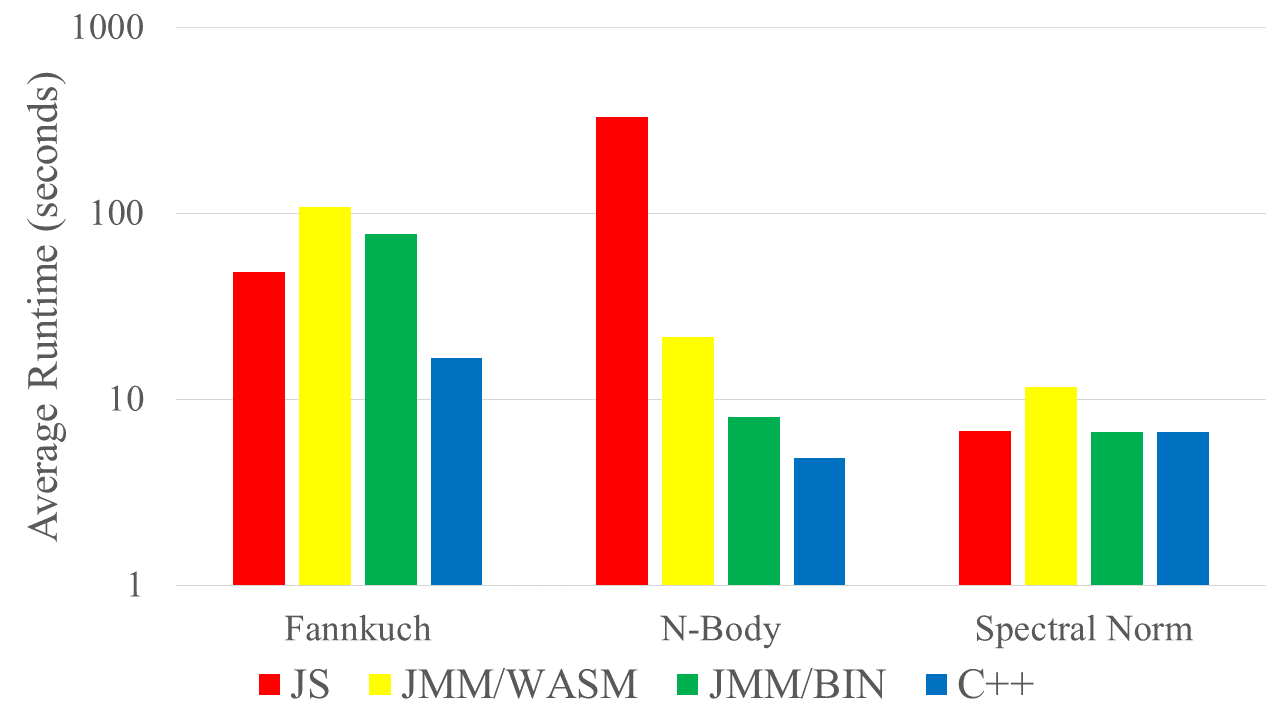
\includegraphics[scale=0.4]{chart.png}
		\caption{Performance of Benchmarks vs. Language and Compiler Target}
	\end{figure}

	Using one-way analysis of variance \cite{Lane}, it was computed for each benchmark that $p < 0.001$, a statistically significant result.
	
	\subsection{Discussion}
	
	In each benchmark, C++ had superior or equal performance to JavaScript and JMM code; the margins in the Fannkuch and N-Body benchmarks were substantial. There is clearly much work ahead before JavaScript matches this performance.
	
	In addition, JMM code compiled to WebAssembly was consistently slower than the same code compiled to native binary. This is likely due to inherent limitations in the current experimental WebAssembly virtual machines and the lack of platform specific optimizations for WebAssembly compilation. Over time, the gap between native and WebAssembly may shrink as WebAssembly improves \cite{Clark2017}. Thus, it is worth comparing performance of JavaScript on V8, a popular JavaScript engine, versus JMM compiled to native, which serves as the performance upper bound of JMM compiled to WebAssembly.
	
	In the Fannkuch benchmark, JavaScript outperforms JMM by nearly 50\%. This benchmark makes use of simple array and numerical operations, which V8 may be able to optimize more effectively. The JMM compiler wraps the vector into the \texttt{\_\_js\_\_Array} struct, which may be the source of JMM's inferior performance.

	For the Spectral Norm benchmark, the performance of all targets except for WebAssembly is equal. That JavaScript is able to match native C++ performance is a testament to the substantial work in browser engineering. It is equally impressive that JMM compiled to native code is able to match the performance of C++. However, as all platforms were equally performant, this benchmark provides little further insight.
	
	Lastly, the N-Body benchmark show substantial performance gains from JMM over JavaScript; native JMM was, on average, 40 times faster than JavaScript! JMM compiled to WebAssembly also outperformed JavaScript by a significant margin. It is unclear what accounts for this huge disparity; it seems improbable to be solely attributable to static typing and manual memory management. Further research is required.

	\section{Conclusion}
	
	JMM shows much promise as a solution for the compilation of JavaScript to WebAssembly. This study has demonstrated that small modifications to existing JavaScript, allowing for compilation to WebAssembly or native code, can lead to substantial performance gains.
	
	Further work on JMM is required to expand the compilable subset of JavaScript enough to include most real world code. The largest difference between JMM and JavaScript is the use of static types; but this difference need not change. Many JavaScript programmers already use type checkers or language supersets that include type checking, both of which prevent bugs \cite{gao2017type}. Moreover, the use of type inference by the JMM compiler enables most well typed JavaScript code to be used with little modification.
	
	Future improvements of JMM must focus on a few critical areas. First, the current memory management model is too restrictive for many existing JavaScript programs to be used unmodified. It may also lead to runtime overhead, as passing the borrow checker sometimes requires unnecessary deep copies. The solution may be using Rust's built-in reference counting system \cite{Klabnik} with a cycle detector to prevent memory leaks. Using a lightweight garbage collector is also worth investigation.
	
	Other JavaScript behavior that JMM does not currently support include JavaScript's objects, which have prototypal inheritance and also serve as untyped hash maps. Another area that must be supported is support for lexical closures, especially for functional expressions. Although these features are not strictly necessary for most tasks, they are quite prevalent and including them would make porting from JavaScript much easier.
	
	Lastly, in order for JMM to truly encompass a usable subset of JavaScript, a much larger set of the standard JavaScript API must be supported, including regular expressions, string and array methods, and mathematics. Tooling that allows for two way interoperation between JavaScript and JMM-generated WebAssembly would also be required for practical use of JMM in the browser.
	
	In addition to new features, performance improvements should certainly be considered. Many improvements will come as WebAssembly VMs mature \cite{Clark2017} and as the Rust compiler adds more optimizations \cite{Matsakis2016}. However, JavaScript specific optimizations should be explored. Pairing the JMM compiler with a JavaScript-to-JavaScript optimizing compiler such as the Google Closure Compiler \cite{ClosureCompiler} or PrePack \cite{prepack} also merits consideration.
	
	JavaScript to WebAssembly compilation shows promise as a source for performance improvements on the web. This study has shown the potential of JMM to make the web faster and thus more accessible for all of its users. The performance of JMM binaries also suggests that JMM may be useful for using JavaScript in embedded systems without the memory overhead of traditional JavaScript engines. Lastly, JMM should be considered as a target for languages that compile to JavaScript; by compiling to JMM, they can achieve significant performance improvements and expedite the transition to WebAssembly.
	
	\newpage
	\bibliographystyle{ieeetr}
	\bibliography{bibliography}
	
\end{document}
